
% xetex expected
\documentclass[xetex,professionalfont]{beamer}

% we want math
\usepackage{amsmath}

% fixes and extensions to amsmath
\usepackage{mathtools}

% additional math symbols
\usepackage{amssymb}

% good-looking fractions in text via \sfrac
\usepackage{xfrac}

% fix spaces after custom commands (see below for examples)
\usepackage{xspace}

% minted allows for fancy syntax highlighting (requires python with pygments)
% usage:
%   \begin{minted}{python}
%   codeb
%   \end{minted}
% \usepackage{minted}

% better looking tables
% usage:
%   begin with a \toprule, write a single row of column headings,
%   then add \midrule and after the columns of data we finish with \bottomrule
% example:
%   \begin{tabular}{llr} \toprule
%   Animal & Description & Price \midrule
%   cat & foo & 10 \\
%   dog & bar & 20 \\ \bottomrule
%   \end{tabular}
% note that good tables generally neither have vertical rules nor double rules
\usepackage{booktabs}

% system font support (requires xetex or luatex)
\usepackage{fontspec}
\setmonofont[Scale=0.7]{Cousine} % part of ttf-chromeos fonts on Arch

% multi-language quotes for babel
\usepackage{csquotes}

% easy way to include copyright information
\usepackage{copyrightbox}

% better bibliographies
\usepackage[backend=biber,style=authoryear]{biblatex}

% language support (english,ngerman)
\usepackage[english]{babel}

% -----------------------------------------------------------------------------

% specify PDF metadata
\hypersetup{pdftitle={CVSP VO - IP Recap},pdfsubject={},pdfauthor={Christopher Pramerdorfer}}

% copyright font style
\makeatletter\renewcommand{\CRB@setcopyrightfont}{\tiny\color{lightgray}}

% add bib file
\addbibresource{literature.bib}

% use tuwcvl beamer theme
\usetheme{tuwcvl}

% -----------------------------------------------------------------------------

% common english abbreviations
\newcommand{\ie}{\mbox{i.e.}\xspace} % i.e.
\newcommand{\eg}{\mbox{e.g.}\xspace} % e.g.

% math - argmin and argmax
\DeclareMathOperator*{\argmin}{arg\,min}
\DeclareMathOperator*{\argmax}{arg\,max}

% shortcuts for number ranges
\newcommand{\NN}{\mathbb{N}}
\newcommand{\ZZ}{\mathbb{Z}}
\newcommand{\QQ}{\mathbb{Q}}
\newcommand{\RR}{\mathbb{R}}

% bold vectors
\renewcommand{\vec}[1]{\ensuremath{\mathbf{#1}}}

% vector shortcuts
\newcommand{\va}{\vec{a}}
\newcommand{\vb}{\vec{b}}
\newcommand{\vc}{\vec{c}}
\newcommand{\ve}{\vec{e}}
\newcommand{\vr}{\vec{r}}
\newcommand{\vs}{\vec{s}}
\newcommand{\vt}{\vec{t}}
\newcommand{\vu}{\vec{u}}
\newcommand{\vv}{\vec{v}}
\newcommand{\vw}{\vec{w}}
\newcommand{\vx}{\vec{x}}
\newcommand{\vy}{\vec{y}}
\newcommand{\vz}{\vec{z}}

\newcommand{\pv}{\ensuremath{\boldsymbol{\theta}}}

% highlight
\newcommand{\highlight}[1]{\textcolor{tuwcvl_inf_red}{\textbf{#1}}}

% -----------------------------------------------------------------------------

\title{Computer Vision Systems Programming VO}
\subtitle{Image Processing Recap}
\author{Christopher Pramerdorfer}
\institute{Computer Vision Lab, Vienna University of Technology}

\begin{document}

% -----------------------------------------------------------------------------

\begin{frame}
\maketitle
\end{frame}

% -----------------------------------------------------------------------------

\begin{frame}
\frametitle{Topics}

Brief \emph{Image Processing} (IP) recap\\\medskip
Assuming you are already familiar with it

\bigskip
\begin{center}
    \copyrightbox[b]
    {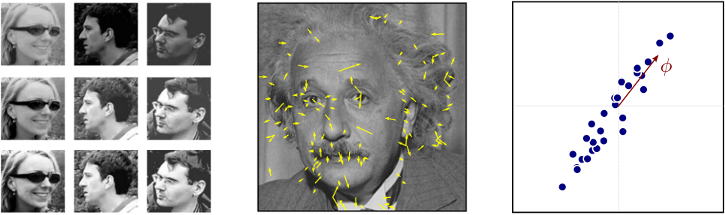
\includegraphics[width=8cm]{figures/intro-collage.png}}
    {\centering Images from \cite{prince12}}
\end{center}

\end{frame}

% -----------------------------------------------------------------------------

\begin{frame}
\frametitle{Image Processing Recap}

We use IP to extract good features from images
\begin{itemize}
    \item Preprocessing step for CV
    \item IP has great influence on CV performance
\end{itemize}

\bigskip
What are good features? More on this later

\bigskip
Let's recap some basic IP methods
\begin{itemize}
    \item No details, this is not an IP lecture
\end{itemize}

\end{frame}

% -----------------------------------------------------------------------------

\begin{frame}
\frametitle{Linear Filtering}

Used for many low-level tasks\\\medskip
Pixel values are linear combination of neighbor values\\\medskip
Computed via \emph{convolution} (or correlation) with kernel $h$ \\\medskip
Different responses depending on kernel

\bigskip
\[
f'(x,y) = \sum_{i,j}f(x-i,y-j)h(i,j) % with convolution the kernel is flipped (x-i,y-j), with correlation this is not the case (x+i,y+j) ... most IP kernels are symmetric so the result is the same
\]

\end{frame}

% -----------------------------------------------------------------------------

\begin{frame}
\frametitle{Linear Filtering}
\framesubtitle{Noise Reduction}

Gain robustness to noise via image blurring\\\medskip
Can be performed by using a 2D Gaussian as kernel $h$ % there are of course others as well
\[
h(i,j)=\frac{1}{2\pi\sigma^2}\exp\left(-\frac{i^2+j^2}{2\sigma^2}\right)
\]

\begin{center}
    \copyrightbox[b]
    {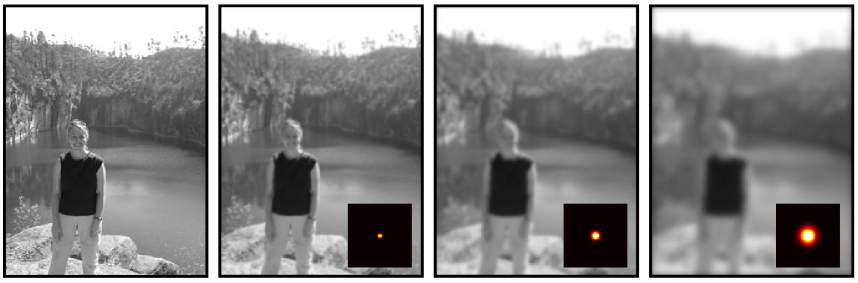
\includegraphics[width=8cm]{figures/linear-blur.png}}
    {\centering Images from \cite{prince12}}
\end{center}

\end{frame}

% -----------------------------------------------------------------------------

\begin{frame}
\frametitle{Linear Filtering}
\framesubtitle{Detecting Brightness Changes -- LoG Filter}

Brightness changes can be valuable information
\begin{itemize}
    \item Object boundaries, textured regions
\end{itemize}

\bigskip
Use a Laplacian of Gaussian (LoG) filter as kernel $h$ % for 3x3 this is just [0 -1 0 ; -1 4 -1 ; 0 -1 0]
\begin{itemize}
    \item Gaussian for noise reduction
    \item Laplacian approximates $\nabla^2=f_{xx}+f_{yy}$ % sum of second unmixed derivatives of image
\end{itemize}

\bigskip
LoG filters respond to intensity changes % strong response near corners, zero crossing on corners
\begin{itemize}
    \item Regardless of direction
    \item At a frequency defined by $\sigma$ of Gaussian
\end{itemize}

\end{frame}

% -----------------------------------------------------------------------------

\begin{frame}
\frametitle{Linear Filtering}
\framesubtitle{Detecting Brightness Changes -- LoG Filter}

Bright and dark regions indicate brightness changes

\bigskip
\begin{center}
    \copyrightbox[b]
    {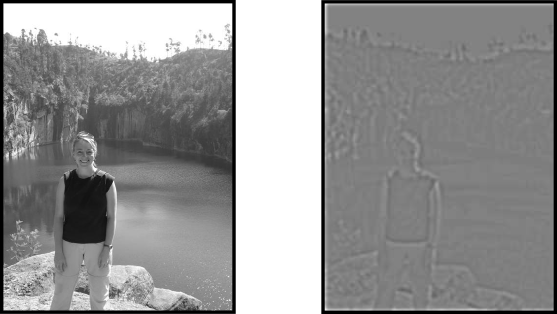
\includegraphics[width=7cm]{figures/linear-log.png}}
    {\centering Images from \cite{prince12}}
\end{center}

\end{frame}

% -----------------------------------------------------------------------------

\begin{frame}
\frametitle{Linear Filtering}
\framesubtitle{Detecting Brightness Changes -- Gabor Filter}

Direction of brightness changes can be valuable
\begin{itemize}
    \item Texture characteristics
\end{itemize}

\bigskip
Use a Gabor filter as kernel $h$, which consists of
\begin{itemize}
    \item A Gaussian for noise reduction
    \item A Sinusoid for change detection 
\end{itemize}

\bigskip
Gabor filters respond to intensity changes at a
\begin{itemize}
    \item Phase and orientation defined by the Sinusoid % phase, orientation, wavelength, but can be made independent of phase by summing squared responses of two filters with pi/2 phase shift
    \item Frequency defined by the Gaussian and Sinusoid
\end{itemize}

\end{frame}

% -----------------------------------------------------------------------------

\begin{frame}
\frametitle{Linear Filtering}
\framesubtitle{Detecting Brightness Changes -- Gabor Filter}

\begin{center}
    \copyrightbox[b]
    {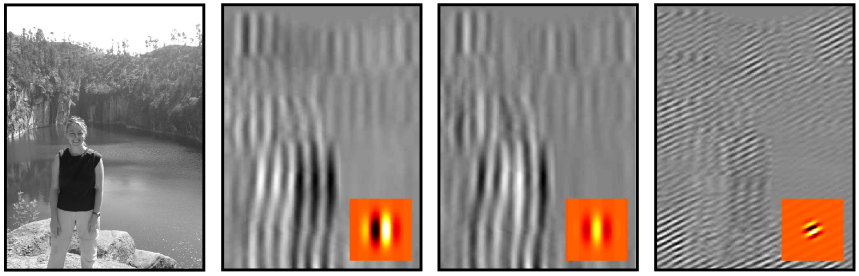
\includegraphics[width=10cm]{figures/linear-gabor.png}}
    {\centering Images from \cite{prince12}}
\end{center}

\end{frame}

% -----------------------------------------------------------------------------

\begin{frame}
\frametitle{Interest Point Detection}

\emph{Interest points} (keypoints) are
\begin{itemize}
    \item Distinctive locations in images
    \item Invariant and robust to image transformations % depending on the type of keypoint
\end{itemize}

\bigskip
Can be detected reliably in multiple images of same object
\begin{itemize}
    \item Used for object detection, structure from motion
\end{itemize}

\end{frame}

% -----------------------------------------------------------------------------

\begin{frame}
\frametitle{Interest Point Detection}
\framesubtitle{SIFT Keypoints}

Scale invariant blob detector
\begin{itemize}
    \item A \emph{blob} is an image region with similar intensity % surrounded by regions with different intensity, again see Tuytelaars08 for more information
\end{itemize}

\bigskip
Blob detection accomplished via LoG filtering
\begin{itemize}
    \item LoG filter responds to blobs of size that depends on $\sigma$
\end{itemize}

\bigskip
Scale invariance is achieved by
\begin{itemize}
    \item Applying LoG filter with multiple $\sigma$
    \item Finding local maxima in resulting scale-space
\end{itemize}

% Repeated LoG approximated by Differences of Gaussians (DoGs)

\end{frame}

% -----------------------------------------------------------------------------

\begin{frame}
\frametitle{Interest Point Detection}
\framesubtitle{SIFT Scale Space}

\begin{center}
    \copyrightbox[b]
    {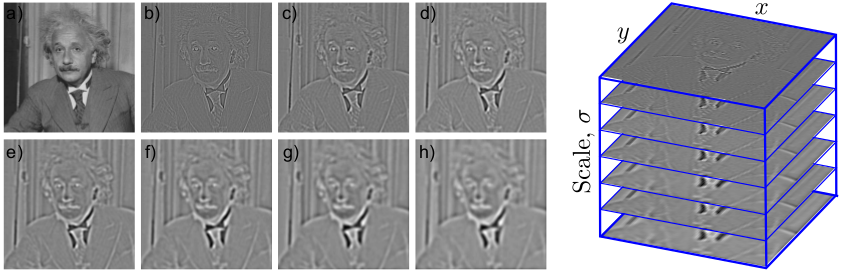
\includegraphics[width=10cm]{figures/sift-scale-space.png}}
    {\centering Images from \cite{prince12}}
\end{center}

\end{frame}

% -----------------------------------------------------------------------------

\begin{frame}
\frametitle{Interest Point Detection}
\framesubtitle{SIFT Keypoints}

Found local maxima are
\begin{itemize}
    \item Discarded unless on image corners
    \item Assigned an orientation via gradient histograms (slide 15) % multiple keypoints are generated if there are more several dominant orientations
\end{itemize}

\bigskip
\begin{center}
    \copyrightbox[b]
    {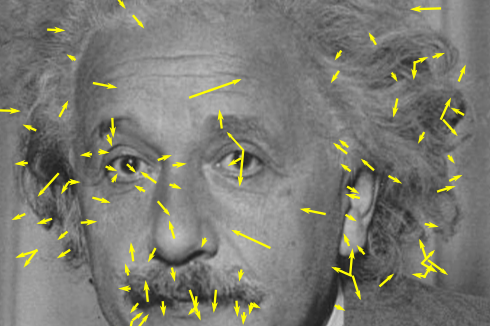
\includegraphics[width=4cm]{figures/ip-sift.png}}
    {\centering Image from \cite{prince12}}
\end{center}

\end{frame}

% -----------------------------------------------------------------------------

\begin{frame}
\frametitle{Local Descriptors}

Compact representations of contents of an image region\\\medskip
Usually computed at interest point locations\\\medskip % but dense representations have uses as well
Invariant in conjunction with suitable interest points\\\medskip % see next slide
Pool information locally to achieve robustness % wrt. small spatial transformations / tradeoff between preserving spatial information and robustness

\end{frame}

% -----------------------------------------------------------------------------

\begin{frame}
\frametitle{Local Descriptors}
\framesubtitle{SIFT Descriptor}

Computed from gradient histograms\\\medskip
Usually used together with SIFT interest points
\begin{itemize}
    \item Compensate for scale, rotation % by transforming image patch by interest point properties before computing descriptors
\end{itemize}

\bigskip
\begin{center}
    \copyrightbox[b]
    {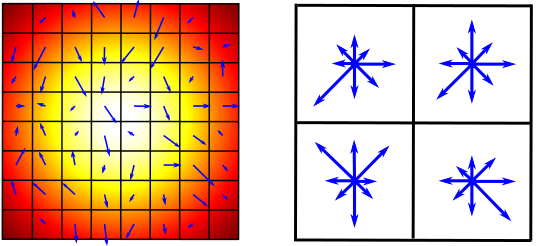
\includegraphics[width=6cm]{figures/sift-descriptor.png}} % divide 8x8 pixel grid into 2x2 cells, pool directions in each cell using a histogram with 8 bins (sift uses 16x16 patches and 4x4 cells, so we have 4x4x8=128 values per descriptor, which is then normalized)
    {\centering Images from \cite{prince12}}
\end{center}

\end{frame}

% -----------------------------------------------------------------------------

\begin{frame}
\frametitle{Local Descriptors}
\framesubtitle{SIFT Descriptor}

SIFT descriptors are
\begin{itemize}
    \item Invariant to scale and rotation (interest points)
    \item Invariant to global intensity changes (gradients)
    \item Robust to small affine transformations (pooling)
\end{itemize}

\end{frame}

% -----------------------------------------------------------------------------

\begin{frame}
\frametitle{Dimensionality Reduction}

Reduce the dimensionality of $\vx$ by removing irrelevant features  % more precisely, if we remove features but leave the reset u, c=color, marker='x', cmap=plt.get_cmap('cool')nchanged, we speak of feature selection. if we compute new features, we speak of feature extraction
\begin{itemize}
    \item Irrelevant means redundant or not discriminative (e.g.\ noise)
\end{itemize}

\bigskip
Advantages
\begin{itemize}
    \item We get a better $\vx$ automatically
    \item Facilitates data visualization  % because we cannot (intuitively) visualize 4+D data
\end{itemize}

\end{frame}

% -----------------------------------------------------------------------------

\begin{frame}
\frametitle{Dimensionality Reduction}
\framesubtitle{PCA}

Assume the following data (30 samples $\vx_1\cdots\vx_{30}$, $\dim(\vx)=2$)
\begin{itemize}
    \item Features are highly correlated
\end{itemize}

\begin{center}
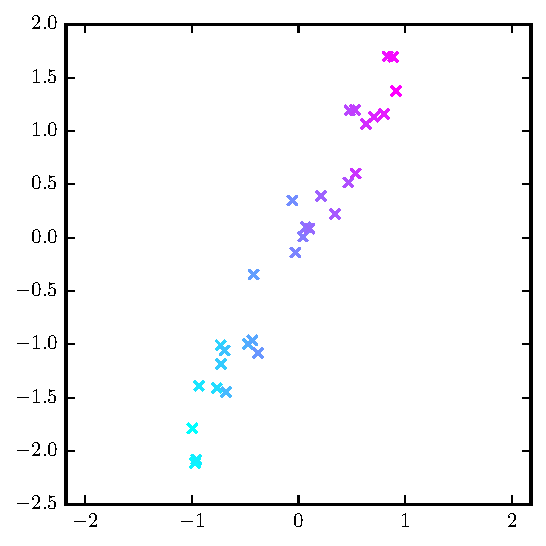
\includegraphics[width=4.5cm]{figures/pca-original.pdf}
\end{center}

\end{frame}

% -----------------------------------------------------------------------------

\begin{frame}
\frametitle{Dimensionality Reduction}
\framesubtitle{PCA}

We want to map the $\vx_k$ to a linear subspace\\\medskip
Spanned by directions of largest data variation

\begin{center}
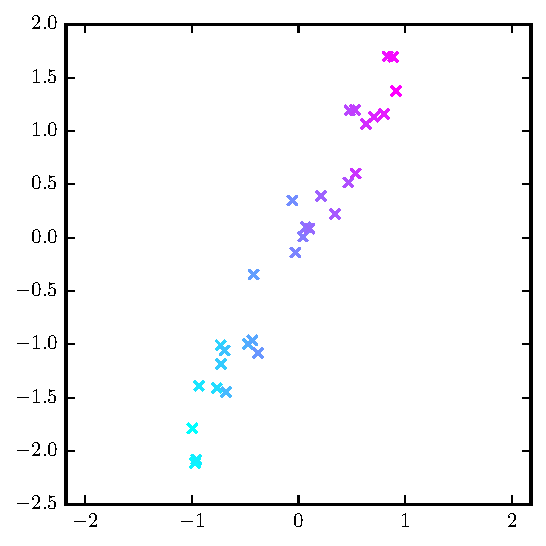
\includegraphics[width=4.5cm]{figures/pca-original.pdf}
\end{center}

\end{frame}

% -----------------------------------------------------------------------------

\begin{frame}
\frametitle{Dimensionality Reduction}
\framesubtitle{PCA}

Standardize individual features (zero mean, unit stddev)\\\medskip  % stddev = standard deviation. stddevs don't have to be 1 but they should be similar, otherwise some features will outweigh others
Compute covariance matrix $\Sigma$
\begin{itemize}
    \item Eigenvectors $\vu_1,\vu_2$ of $\Sigma$ are sought direction vectors
\end{itemize}

\begin{center}
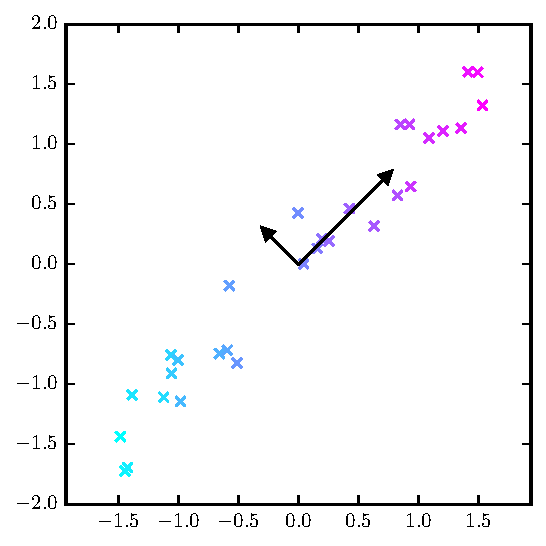
\includegraphics[width=4.5cm]{figures/pca-eigenvectors.pdf}
\end{center}

\end{frame}

% -----------------------------------------------------------------------------

\begin{frame}
\frametitle{Dimensionality Reduction}
\framesubtitle{PCA}

Represent $\vx_k$ in the $U=(\vu_1,\vu_2)$ basis, $\vx^r_k=U^\top\vx_k$
\begin{itemize}
    \item $\vu_1,\vu_2$ are orthogonal, so $U$ is a rotation matrix % because sigma is symmetric
\end{itemize}

\begin{center}
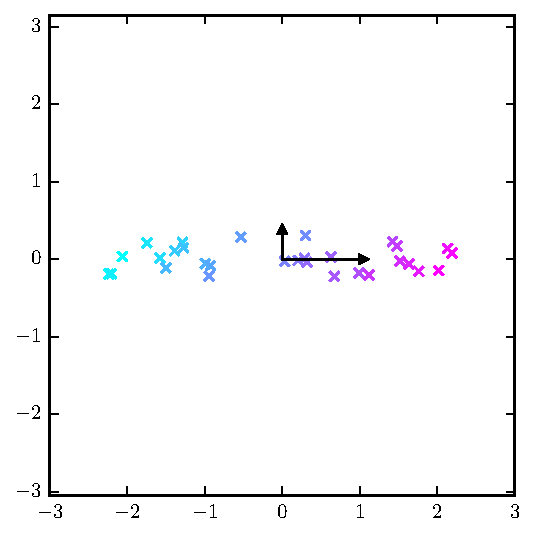
\includegraphics[width=4.5cm]{figures/pca-rotated.pdf}
\end{center}

\end{frame}

% -----------------------------------------------------------------------------

\begin{frame}
\frametitle{Dimensionality Reduction}
\framesubtitle{PCA}

Now we can simply drop features that vary little  % this is visualized here by setting them to 0
\begin{itemize}
    \item Encoded by the corresponding eigenvalues $\lambda_1,\lambda_2$
\end{itemize}

\begin{center}
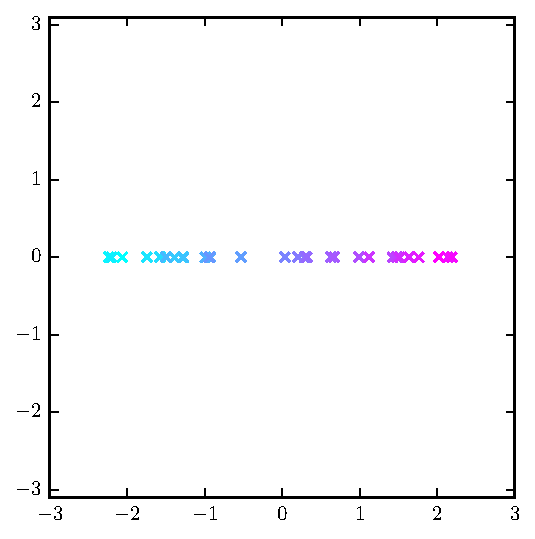
\includegraphics[width=4.5cm]{figures/pca-reduced.pdf}
\end{center}

\end{frame}

% -----------------------------------------------------------------------------

\begin{frame}
\frametitle{Dimensionality Reduction}
\framesubtitle{PCA}

If desired we can approximate $\vx_k$ by multiplying with $U$  % after padding with zeros of course

\begin{center}
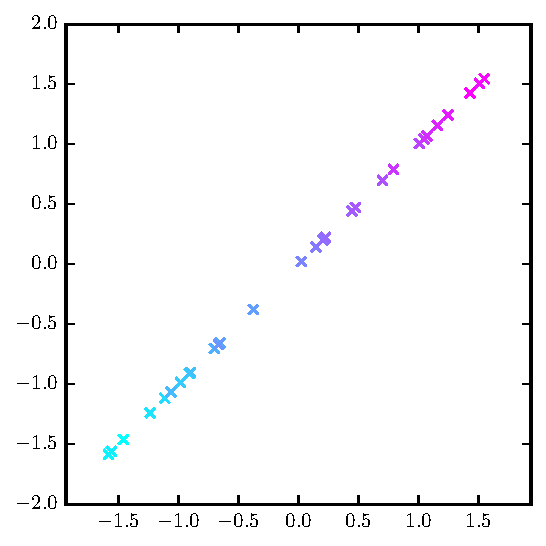
\includegraphics[width=4.5cm]{figures/pca-reconstructed.pdf}
\end{center}

\end{frame}

% -----------------------------------------------------------------------------

\begin{frame}
\frametitle{Dimensionality Reduction}
\framesubtitle{PCA}

This method is called \emph{Principal Component Analysis (PCA)}

\bigskip
Used to find features that retain e.g.\ 99\% of variance
\begin{itemize}
    \item Often leads to a significant dimensionality reduction
\end{itemize}

\bigskip
Used to perform \emph{whitening} % to do so we simply rotate the x as before and then divide them by the square root of the corresponding eigenvalues. this results in unit variance
\begin{itemize}
    \item To obtain uncorrelated features with same variance % features extracted via pca are uncorrelated as the data were projected onto orthogonal eigenvectors
    \item Needed by some ML algorithms
\end{itemize}

\end{frame}

% -----------------------------------------------------------------------------

\begin{frame}
\frametitle{Bibliography}

\printbibliography

\end{frame}

\end{document}
